%% =====================================================================
\section{System Model}\label{sec:model}
%% =====================================================================
\subsection{Network and Scenario}\label{sec:story}
We consider a UAV that flies over a disaster area and reports to a ground station (GS) that coordinates the response, as shown in Fig.~\ref{fig:system}. Time is divided into slots of length $\tau$, indexed by $t\in\{0,1,\dots\}$. The UAV flies at constant speed along a route planned before the mission, so its position $\mathbf{u}(t)$ in every slot is known in advance. In each slot the UAV photographs the patch of ground below it, which we call its footprint, and a small classifier on board decides whether an event of interest is present in the patch, for example flooding, fire, a collapsed building or a survivor. Throughout the paper we use flood mapping as the running example: the classifier labels each photo ``flooded'' or ``dry'', and the response teams need to know which patches are under water. The model applies to any such event with a suitable classifier.

Since the UAV moves, the patch below it changes from slot to slot, and consecutive footprints partly overlap. We do not model the whole area. We model only what the UAV sees along its route: in slot $t$, $X(t)$ is the state of the patch below the UAV and $Y(t)$ is the photo of that patch. The position $\mathbf{u}(t)$ affects the model in one place only, the link to the GS. The distance and the elevation angle to the GS determine how likely a packet is to arrive and how much energy it costs. The route can have any shape. In our evaluation it is a circle, so the UAV passes alternately through parts of the route close to the GS and far from it.

The GS has no sensor of its own. Everything it knows about the patch below the UAV comes from the UAV. We call the GS status the label that the GS currently holds for this patch: it is the last label the GS received, either a label sent by the UAV or the label that a larger classifier at the GS produced from a photo sent by the UAV. The GS holds this status until the next update arrives, and the response teams act on it. In each slot the UAV can therefore stay silent, send its on-board label, or send the photo. A label is a few bytes and cheap to send, but it may be wrong. A photo is tens of kilobytes and much more expensive, and it may fail to arrive far from the GS, but the ground classifier labels it almost always correctly. The UAV chooses under an energy budget and without observing the true state. Table~\ref{tab:notation} summarizes the notation.

\begin{figure}[t]
\centering
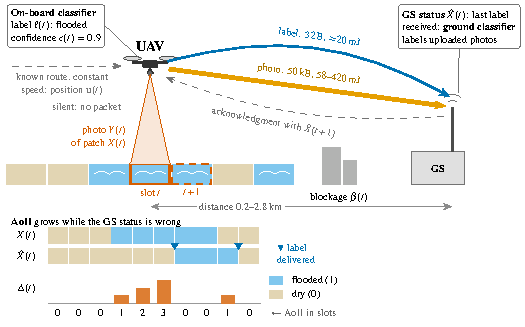
\includegraphics[width=\columnwidth]{figures/fig_scenario.pdf}
\caption{The scenario. A UAV flies over a disaster area (flooding in this example), photographs the patch below it and labels the photo on board with a confidence. In each slot it stays silent, sends its label (blue), or sends the photo to the ground classifier (orange). The GS status is the last label received, and every packet is acknowledged with it. Buildings can block the link, and the cost of a photo grows with the distance. Inset: the AoII grows by one per slot while the GS status is wrong and returns to zero when a delivered label or a change of the scene makes it right.}
\label{fig:system}
\end{figure}

\begin{table}[t]
\caption{Main notation}\label{tab:notation}
\centering\footnotesize
\setlength{\tabcolsep}{3pt}
\begin{tabular}{@{}p{0.52\columnwidth}ll@{}}
\toprule
Meaning & Symbol & Defined in\\
\midrule
Patch below the UAV: event or not & $X(t)$ & \eqref{eq:source}\\
How often the scene changes & $p_0,p_1$; $\varpi$ & \eqref{eq:source}, \eqref{eq:stationary}\\
Photo; on-board label, confidence & $Y(t)$; $\lab(t)$, $c(t)$ & \eqref{eq:calib}\\
Label disagrees with the GS status & $d(t)$ & Sec.~\ref{sec:belief}\\
Label from the ground classifier & $\lab^{\rm g}(t)$, $\ee_{\rm g}(c)$ & Assum.~\ref{as:inf}\\
Silent, send label, send photo & $a(t)\in\{0,1,2\}$ & Sec.~\ref{sec:act}\\
UAV position, blockage & $g(t)$ & \eqref{eq:block}, \eqref{eq:pl}\\
Packet decoded & $o(t)$ & \eqref{eq:est}\\
Delivery probability; energy & $q_a(g)$; $E_a(g)$ & \eqref{eq:succ}, \eqref{eq:energy}\\
Energy budget of the mission & $\bar E$ & \eqref{eq:budget}\\
What the GS status says & $\hat X(t)$ & \eqref{eq:est}\\
How long the GS status has been wrong & $\Delta(t)$ (AoII) & \eqref{eq:aoii}\\
What the UAV believes about $\Delta(t)$ & $\pi_t$; $\mu_t$, $S_t$ & \eqref{eq:belief}, \eqref{eq:musum}\\
Evidence of a frame that the GS is wrong & $\Lambda_t$ & \eqref{eq:Lambda}\\
Value of an action; its energy price & $G_a$; $Z(t)$, $V$ & Secs.~\ref{sec:structure}, \ref{sec:lyap}\\
\bottomrule
\end{tabular}
\end{table}

\subsection{Event Dynamics}\label{sec:src}
\begin{figure}[t]
\centering
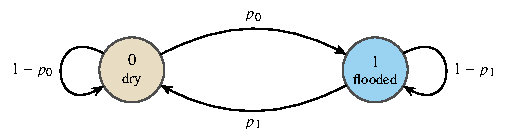
\includegraphics[width=0.7\columnwidth]{figures/fig_markov.pdf}
\caption{Markov chain of the patch state $X(t)$. In each slot a dry patch ($0$) is followed by a flooded one with probability $p_0$, and a flooded patch ($1$) by a dry one with probability $p_1$. On our flood data $p_0=0.039$ and $p_1=0.166$.}
\label{fig:markov}
\end{figure}
We describe the patch below the UAV by a binary state $X(t)\in\{0,1\}$, with $X(t)=1$ if the event is present and $X(t)=0$ otherwise. In the flood example, $X(t)=1$ means that the patch is flooded. The UAV moves a short distance between slots, so consecutive frames cover overlapping areas and the state tends to persist: a flooded footprint is usually followed by another flooded footprint. Note that $X(t)$ refers to the patch below the UAV in slot $t$, not to a fixed patch. The chain therefore describes how the state changes from one footprint to the next along the route, and its transition probabilities depend on the speed of the UAV and on the overlap of its footprints. They are constant because the speed is. The simplest model that captures this persistence is the two-state Markov chain of Fig.~\ref{fig:markov}. Let $p_x$ be the probability that the state leaves $x$ in one slot,
\begin{equation}\label{eq:source}
\Prob\big\{X(t+1)\neq x\mid X(t)=x\big\}=p_x,\qquad x\in\{0,1\}.
\end{equation}
We assume $0<p_0,p_1<\tfrac12$. The lower bound makes the chain irreducible, so the scene does change and every state is visited. The upper bound says that the state is more likely to stay than to change in one slot. This persistence is what makes an old status useful at all: if the state changed more often than not, the GS would do better by inverting its last label than by keeping it. We use the bound $p_x<\frac12$ in Section~\ref{sec:structure}.

The fraction of time the chain spends in each state follows from the balance between the two transitions. In steady state the probability flow from 0 to 1 equals the flow from 1 to 0, so $\varpi_0p_0=\varpi_1p_1$, and with $\varpi_0+\varpi_1=1$,
\begin{equation}\label{eq:stationary}
\varpi_1=\frac{p_0}{p_0+p_1},\qquad \varpi_0=\frac{p_1}{p_0+p_1}.
\end{equation}
We call $\varpi=(\varpi_0,\varpi_1)$ the class prior. The chain may be asymmetric. In our flood data a flooded footprint turns dry more often than a dry one floods ($p_0=0.039$, $p_1=0.166$), so only $\varpi_1=19\%$ of the footprints are flooded. We use the symmetric case $p_0=p_1$ only to state some results in a simpler form.

\subsection{On-Board and Ground Classification}
In slot $t$ the UAV takes a photo $Y(t)$ of the patch below it, which we also call a frame. The photo is used only to classify the patch; the UAV knows its position from the route and does not infer it from the photo. The on-board classifier returns a label and a confidence,
\begin{equation}\label{eq:label}
\lab(t)\in\{0,1\},\qquad c(t)\in[\tfrac12,1],
\end{equation}
where $\lab(t)$ is the state that the classifier finds more likely and $c(t)$ is the probability it assigns to that state. A classifier that outputs a probability $p$ of flooding, as most do, gives $\lab(t)=\ind{p\ge\frac12}$ and $c(t)=\max\{p,1-p\}$. The confidence is useful only if it means what it says. We therefore require that the classifier be calibrated: among all frames that receive label $\lab$ and confidence $c$, a fraction $c$ is truly in state $\lab$, for both label values,
\begin{equation}\label{eq:calib}
\Prob\big\{X(t)=\lab(t)\mid\lab(t),\,c(t)\big\}=c(t).
\end{equation}
Averaging~\eqref{eq:calib} over the two label values shows that a label with confidence $c$ is wrong with probability $1-c$. The converse does not hold. A classifier can have this property while being overconfident when it says ``flooded'' and underconfident when it says ``dry''. We need~\eqref{eq:calib} for each label value because the belief update below uses the probability of each state given the label, and flooded and dry patches are not equally common.

Modern classifiers are often overconfident, so~\eqref{eq:calib} does not hold out of the box. Post-hoc calibration~\cite{guo2017calibration}, such as isotonic regression on held-out data, restores it to a good approximation. Fig.~\ref{fig:inference}(a) shows that our on-board model, calibrated in this way, has an expected calibration error of $1.4\%$ on the test chips. Fig.~\ref{fig:inference}(b) confirms the consequence above: the measured error rate of the on-board label follows $1-c$ closely across confidence bins.

The belief update in Section~\ref{sec:belief} needs the likelihood of a frame under each state, that is, how much more probable the observed pair $(\lab(t),c(t))$ is if $X(t)=1$ than if $X(t)=0$. Calibration gives the posterior probability of each state, not the likelihood. By~\eqref{eq:calib}, the posterior probability of state $x\in\{0,1\}$ is
\begin{equation}\label{eq:cx}
c_x(t)=\Prob\big\{X(t)=x\mid\lab(t),c(t)\big\}=\begin{cases}c(t), & x=\lab(t),\\ 1-c(t), & x\neq\lab(t).\end{cases}
\end{equation}
By Bayes' rule and~\eqref{eq:cx}, posterior and likelihood are related through the class prior,
\begin{equation}\label{eq:lik}
\Prob\big\{\lab(t),c(t)\mid X(t)=x\big\}=\frac{c_x(t)\,\Prob\big\{\lab(t),c(t)\big\}}{\varpi_x}\propto\frac{c_x(t)}{\varpi_x},
\end{equation}
since the factor $\Prob\{\lab(t),c(t)\}$ does not depend on $x$. The division by $\varpi_x$ matters when the classes are unbalanced. A frame with confidence $c(t)=0.5$, for example, looks neutral, but since only $19\%$ of the footprints are flooded, it is $(0.5/0.19)/(0.5/0.81)\approx4.3$ times more likely under $X=1$ than under $X=0$. The classifier has already used the prior to produce its output, and the belief update below uses the source dynamics, which contain the same prior. Dividing by $\varpi_x$ prevents counting the prior twice.

After a raw upload, the ground classifier labels the frame. We denote its label by $\lab^{\rm g}(t)$ and its error probability by $\ee_{\rm g}$. The ground model is larger and sees all spectral bands, so it is more accurate than the on-board model. Its errors are not independent of the on-board confidence, however: frames that are hard on board are often hard on the ground as well. In our data the ground model errs on $20\%$ of the frames that the on-board model gets wrong and on $0.8\%$ of the others. Fig.~\ref{fig:inference}(b) shows the ground error rate as a function of the on-board confidence: it is about $8\%$ for $c<0.8$ and falls to about $1\%$ for $c>0.95$. We therefore let the ground error depend on the on-board confidence and write $\ee_{\rm g}(c)$.

\begin{figure*}[t]
\centering
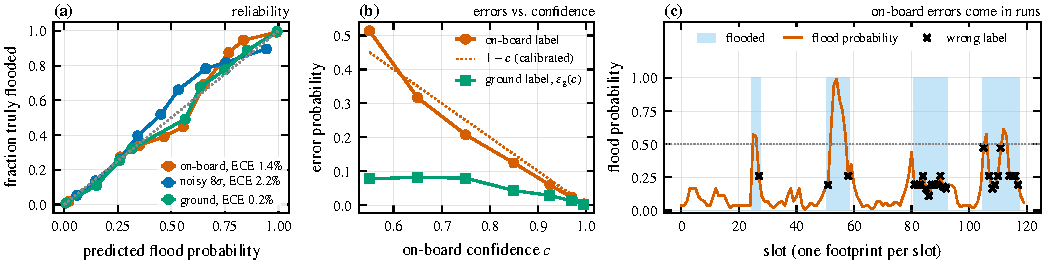
\includegraphics[width=\textwidth]{figures/fig_inference.pdf}
\caption{Inference traces on the Sen1Floods11 test chips. (a) Reliability diagram: fraction of flooded footprints versus the calibrated probability of flooding, for the on-board model, its noisiest variant (input noise of $8$ standard deviations), and the ground model, with expected calibration errors (ECE) in parentheses. (b) Error probability of the on-board label and of the ground label versus the on-board confidence $c$; the dotted line is $1-c$, which a calibrated model follows. (c) A segment of $120$ consecutive footprints of one test chip: flooded footprints are shaded, the line is the on-board flood probability, and the on-board errors (crosses) come in runs, mostly when a flooded area is missed.}
\label{fig:inference}
\end{figure*}

We collect these modeling choices in an assumption. It is used only to design the controller; the simulations in Section~\ref{sec:results} replay real classifier outputs, which do not satisfy it exactly.

\begin{assumption}[Inference model]\label{as:inf}
(i) The on-board classifier is calibrated, i.e.,~\eqref{eq:calib} holds. (ii) Given the source path, the on-board outputs $(\lab(t),c(t))$ are independent across slots. (iii) Given $X(t)$ and $c(t)=c$, the ground label is wrong with probability $\ee_{\rm g}(c)<\tfrac12$, independently of $\lab(t)$ and of the past.
\end{assumption}

Part (ii) is the strongest of the three. Consecutive footprints overlap by half, so a feature that fools the classifier in one frame tends to fool it in the next. Fig.~\ref{fig:inference}(c) shows such runs of errors. Over the validation and test chips, the on-board label is wrong in $8.2\%$ of the slots, but in $56\%$ of the slots that follow a wrong label, and a run of errors lasts $2.2$ slots on average. We keep part (ii) because it yields a tractable belief update, and we correct for its optimism in Section~\ref{sec:belief}. Assumption~\ref{as:inf} generalizes the semantic-noise model of Tiny-SEM~\cite{hosny2026tinysem}, in which the noise level is the same for every sample.

\subsection{Actions and Channel}\label{sec:act}
At the start of slot $t$, after classifying the frame, the UAV chooses an action $a(t)\in\A=\{0,1,2\}$. It stays silent ($a=0$), which costs nothing and leaves the GS status unchanged. It sends its label in a packet of $L_1$ bits ($a=1$), which corrects a wrong GS status if the label is right but makes a correct status wrong if the label is wrong. Or it uploads the frame in a packet of $L_2\gg L_1$ bits ($a=2$), so that the ground classifier labels it. In our scenario a label packet has $32$ bytes and a frame $50$ kilobytes. Whether a packet arrives, and how much energy it costs, depends on the link, which we model next.

Whether a packet arrives depends on the link state $g(t)=(\mathbf{u}(t),\beta(t))$. The first part is the position $\mathbf{u}(t)$ of the UAV on its route, which is known in advance because the route and the speed are fixed. The second part is a blockage indicator $\beta(t)\in\{0,1\}$. Buildings and terrain block the link for several slots at a time, so we model $\beta(t)$ as a two-state Markov chain with
\begin{equation}\label{eq:block}
\begin{split}
\Prob\big\{\beta(t+1)=1\mid\beta(t)=0\big\}&=\rho_{\rm b},\\
\Prob\big\{\beta(t+1)=0\mid\beta(t)=1\big\}&=\rho_{\rm u}.
\end{split}
\end{equation}
A blockage then lasts $1/\rho_{\rm u}$ slots on average, and a fraction $\rho_{\rm b}/(\rho_{\rm b}+\rho_{\rm u})$ of the slots is blocked. No packet gets through a blocked link.

When the link is not blocked, the received power depends on the distance $r$ between the UAV and the GS and on the elevation angle $\phi$. A low UAV is often seen through buildings, so the link is in line of sight (LoS) only with some probability. Following~\cite{alhourani2014lap}, we use the mean path loss
\begin{equation}\label{eq:pl}
\overline{\rm PL}(r,\phi)={\rm FSPL}(r)+P_{\rm LoS}(\phi)\,\eta_{\rm LoS}+\big(1-P_{\rm LoS}(\phi)\big)\eta_{\rm NLoS},
\end{equation}
where ${\rm FSPL}(r)$ is the free-space path loss, $\eta_{\rm LoS}$ and $\eta_{\rm NLoS}$ are the excess losses in LoS and non-LoS, and $P_{\rm LoS}(\phi)=[1+\alpha e^{-b(\phi-\alpha)}]^{-1}$ grows with the elevation angle, with environment constants $\alpha$ and $b$. The transmit power, the path loss~\eqref{eq:pl}, the bandwidth $W$ and the receiver noise figure give the mean signal-to-noise ratio (SNR) $\bar\gamma(g)$.

Small-scale fading makes the instantaneous SNR random around this mean. With Rayleigh fading, the instantaneous SNR is $\bar\gamma(g)\,|h|^2$ with $|h|^2$ exponentially distributed with unit mean. The fading coefficient $h$ stays constant during a slot. The UAV sends a packet of $L_a$ bits with a rateless (incremental-redundancy) code: it keeps sending coded bits until the GS decodes the packet and acknowledges it, or until a transmission window $\tau_{\max}\le\tau$ ends. Decoding takes the time $L_a/C(h)$, where $C(h)=W\log_2(1+\bar\gamma|h|^2)$ is the capacity of the faded channel, so the packet is decoded if $L_a/C(h)\le\tau_{\max}$, that is, if $W\tau_{\max}\log_2(1+\bar\gamma|h|^2)\ge L_a$. Solving for $|h|^2$ gives the delivery probability
\begin{equation}\label{eq:succ}
q_a(g)=(1-\beta)\,\exp\!\Big(-\frac{\gamma_a}{\bar\gamma(g)}\Big),\qquad \gamma_a=2^{L_a/(W\tau_{\max})}-1,
\end{equation}
for $a\in\{1,2\}$,
and $q_0\equiv0$. Here $\gamma_a$ is the SNR needed to deliver $L_a$ bits within the window. Since $L_2>L_1$, $\gamma_2>\gamma_1$, so $q_2(g)\le q_1(g)$ in every link state. In our scenario a label gets through almost surely whenever the link is not blocked, while a raw frame succeeds with probability between $0.99$ near the GS and $0.25$ at the far end of the trajectory.

The link is therefore an erasure channel: a packet either arrives intact or is lost, and a lost packet leaves the GS status unchanged. The link never changes the content of a label. Every packet carries a $32$-bit cyclic redundancy check (CRC), and the GS discards a packet whose check fails; a corrupted packet passes with probability about $2^{-32}$. We also assume that acknowledgments, which are short and sent by the GS at higher power, always arrive.

\begin{remark}[Undetected errors]\label{rem:flip}
Suppose instead that a decoded label is flipped with a small probability $\ee_{\rm u}$. Because the label is binary, a flipped disagreeing label equals the current GS status, so it changes nothing. A bit error on the link can therefore cancel an update but cannot make a correct GS status wrong. Its only effect is to replace $q_1(g)$ by $q_1(g)(1-\ee_{\rm u})$ in everything that follows. An undetected error in a raw frame corrupts the photo rather than the label, and its effect can be folded into the ground error $\ee_{\rm g}(c)$.
\end{remark}

\subsection{Energy Consumption}
A transmission costs the energy of the radio while it transmits plus a fixed overhead per packet. With the rateless code above, the radio is on for $\min\{L_a/C(h),\tau_{\max}\}$, so the expected energy of action $a$ is $P_{\rm r}\,\E_h\big[\min\{L_a/C(h),\tau_{\max}\}\big]+E_{\rm o}$. The controller needs this value before it transmits, when $h$ is unknown, and we approximate it by evaluating the airtime at the mean rate $\bar R(g)=W\log_2(1+\bar\gamma(g))$:
\begin{equation}\label{eq:energy}
E_a(g)=P_{\rm r}\min\Big\{\frac{L_a}{\bar R(g)},\tau_{\max}\Big\}+E_{\rm o},\quad a\in\{1,2\},
\end{equation}
and $E_0=0$. Here $P_{\rm r}$ is the power drawn by the radio and $E_{\rm o}$ is the overhead of waking up the radio, accessing the channel and receiving the acknowledgment. In our scenario a label costs about $20$\,mJ, almost all of it overhead, while a raw frame costs between $58$\,mJ and $420$\,mJ depending on the distance. Averaging over the fading instead gives $20$ to $22$\,mJ for a label and $64$ to $395$\,mJ for a raw frame along our trajectory. The approximation~\eqref{eq:energy} is thus accurate for labels and within $-30\%$ to $+12\%$ of the exact value for raw frames; it underestimates the cost of a raw frame most at intermediate distances, where a deep fade can extend the transmission to the full window. Capture, inference and propulsion~\cite{zeng2019rotary} cost the same whatever the decision, so we constrain only the communication energy, through a long-run average budget of $\bar E$ joules per slot:
\begin{equation}\label{eq:budget}
\limsup_{T\to\infty}\frac1T\sum_{t=0}^{T-1}\E\Big[E_{a(t)}\big(g(t)\big)\Big]\le\bar E.
\end{equation}
The expectation is over the action and the link state, which are random: they depend on the scene, the classifier outputs, the blockage and the past deliveries. Since $E_a(g)$ already averages over the fading, \eqref{eq:budget} limits the long-run average energy that the radio draws, up to the approximation error of~\eqref{eq:energy}. The $\limsup$ is needed because the running average need not converge for every policy. An average budget allows the UAV to spend more in some parts of the mission, for example near the GS where uploads are cheap, and less in others.

\subsection{The GS Status and the AoII}
Let $o(t)\in\{0,1\}$ indicate that the packet sent in slot $t$ is decoded, so $\Prob\{o(t)=1\mid a(t)=a,g(t)=g\}=q_a(g)$. The GS status, which we denote by $\hat X(t)$, is the most recent label the GS has received, whether it came from the UAV or from the ground classifier:
\begin{equation}\label{eq:est}
\hat X(t+1)=\begin{cases}\lab(t), & a(t)=1,\ o(t)=1,\\ \lab^{\rm g}(t), & a(t)=2,\ o(t)=1,\\ \hat X(t), & \text{otherwise.}\end{cases}
\end{equation}
Holding the last label is the natural estimator when the state is persistent ($p_x<\frac12$). The GS acknowledges every decoded packet and includes the new status $\hat X(t+1)$ in the acknowledgment, which costs one byte. The UAV therefore always knows $\hat X(t)$. It never knows $X(t)$.

The GS status can be wrong for two reasons. The scene may change, for example when the UAV passes from flooded patches to dry ones, while the GS keeps the old status until the UAV updates it. Or the update itself may be wrong: the small on-board classifier mislabels some photos, especially ambiguous ones such as a dry field after rain, and a wrong label that reaches the GS turns a correct status into a wrong one. What matters to the response teams is how long the status has been wrong: a status that is wrong for one slot does little harm, while one that is wrong for a minute may send a team to the wrong place. We therefore measure how well the GS knows the scene by the AoII~\cite{maatouk2020aoii}. The AoII is zero while the GS status is correct and counts the slots for which it has been wrong otherwise. After the scene moves to $X(t+1)$, it evolves as
\begin{equation}\label{eq:aoii}
\Delta(t+1)=\big(\Delta(t)+1\big)\,\ind{X(t+1)\neq\hat X(t+1)},\quad \Delta(0)=0.
\end{equation}
The AoII captures two effects that the AoI misses. A delivered wrong label makes a correct GS wrong, so the AoII starts to grow right after a delivery. A GS that has been wrong for a long time is penalized more than one that has just become wrong, which favors correcting long errors first.

Table~\ref{tab:aoiiex} gives an example from the flood scenario over eight slots. In slot $2$ a wrong ``flooded'' label is delivered, so the GS becomes wrong in slot $3$ although the scene has not changed. In slot $4$ the patch floods, and the GS happens to become correct. In slot $4$ the UAV also delivers a wrong ``dry'' label, so the GS is wrong again in slots $5$ and $6$, until a correct label sent in slot $6$ fixes it.

\begin{table}[t]
\caption{AoII in a flood example ($1$: flooded, $0$: dry)}\label{tab:aoiiex}
\centering\footnotesize
\setlength{\tabcolsep}{5pt}
\begin{tabular}{@{}lcccccccc@{}}
\toprule
Slot $t$ & 1 & 2 & 3 & 4 & 5 & 6 & 7 & 8\\
\midrule
True state $X(t)$ & 0 & 0 & 0 & 1 & 1 & 1 & 1 & 1\\
Delivered label in slot $t$ & -- & 1 & -- & 0 & -- & 1 & -- & --\\
GS status $\hat X(t)$ & 0 & 0 & 1 & 1 & 0 & 0 & 1 & 1\\
AoII $\Delta(t)$ & 0 & 0 & 1 & 0 & 1 & 2 & 0 & 0\\
\bottomrule
\end{tabular}
\end{table}

The AoII is random, since the scene, the on-board errors and the deliveries are, and it depends on the true state, which the UAV never observes. Section~\ref{sec:problem} therefore takes its long-run average as the objective and replaces it with a belief that the UAV can compute.

\subsection{Order of Events}\label{sec:events}
Within slot $t$, events occur in the following order.
\begin{enumerate}
\item The UAV observes the link state $g(t)$, captures $Y(t)$ and computes $\lab(t)$ and $c(t)$.
\item It chooses $a(t)$ and transmits if $a(t)\neq0$.
\item The packet is decoded with probability $q_{a(t)}(g(t))$. If it is, the GS updates its status by~\eqref{eq:est} and sends the acknowledgment.
\item The scene moves to $X(t+1)$, and the AoII becomes $\Delta(t+1)$ by~\eqref{eq:aoii}.
\end{enumerate}
